\documentclass[11pt]{article}
\usepackage{geometry}
\geometry{letterpaper}

\usepackage{graphicx}
\usepackage{amssymb}
\usepackage{epstopdf}
\usepackage{natbib}
\usepackage{amssymb, amsmath}
\DeclareGraphicsRule{.tif}{png}{.png}{`convert #1 `dirname #1`/`basename #1 .tif`.png}
\graphicspath{{images/} }%{./}} %put all Figures in these dirs

\usepackage[colorinlistoftodos]{todonotes}
\usepackage{hyperref}
\usepackage{xcolor}
\hypersetup{
    colorlinks,
    linkcolor={black},
    citecolor={blue!30!black},
    urlcolor={blue!50!black}
}
\usepackage{pdfpages}
\usepackage[small, labelfont=bf]{caption}
\usepackage{subcaption}

\renewcommand\bibsection{%
   \section{References}%
}%
\usepackage{comment}

\title{Social discovery and its impact on the spread of infectious diseases}
\author{Arnold Steffen, Cadow Joris}
%\date{date}

\begin{document}



\thispagestyle{empty}

\begin{center}

\includegraphics[width=5cm]{ETHlogo.eps}

\bigskip


\bigskip


\bigskip


\LARGE{ 	Lecture with Computer Exercises:\\ }
\LARGE{ Modelling and Simulating Social Systems with MATLAB\\}

\bigskip

\bigskip

\small{Project Report}\\

\bigskip

\bigskip

\bigskip

\bigskip


\begin{tabular}{c}
%\hline
\\
\textbf{\LARGE{Social discovery and its impact on }}\\
\textbf{\LARGE{the spread of infectious diseases}}\\
\\
%\hline
\end{tabular}
\bigskip

\bigskip

\bigskip

\LARGE{Steffen Arnold \& Joris Cadow}



\bigskip

\bigskip

\bigskip

\bigskip

\bigskip

\bigskip

\bigskip

\bigskip

Z\"urich\\
December 2015\\

\end{center}

\newpage

%%%%%%%%%%%%%%%%%%%%%%%%%%%%%%%%%%%%%%%%%%%%%%%%%

\newpage
\section*{Agreement for free-download}
\bigskip


\bigskip


\large We hereby agree to make our source code for this project freely available for download from the web pages of the SOMS chair.
%It can also be found on \href{https://github.com/verticube/msssm}{GitHub}\footnote{https://github.com/verticube/msssm}.
Furthermore, we assure that all source code is written by ourselves and is not violating any copyright restrictions.


\begin{center}

\bigskip


\bigskip


\begin{tabular}{@{}p{3.3cm}@{}p{6cm}@{}@{}p{6cm}@{}}
\begin{minipage}{3cm}

\end{minipage}
&
\begin{minipage}{6cm}
\vspace{5mm} \large Steffen Arnold

 \vspace{\baselineskip}

\end{minipage}
&
\begin{minipage}{6cm}

\large Joris Cadow

\end{minipage}
\end{tabular}


\end{center}
\newpage

%%%%%%%%%%%%%%%%%%%%%%%%%%%%%%%%%%%%%%%

\includepdf{./declaration-originality.pdf}


% IMPORTANT
% you MUST include the ETH declaration of originality here; it is available for download on the course website or at http://www.ethz.ch/faculty/exams/plagiarism/index_EN; it can be printed as pdf and should be filled out in handwriting


%%%%%%%%%% Table of content %%%%%%%%%%%%%%%%%

\tableofcontents

\newpage

%%%%%%%%%%%%%%%%%%%%%%%%%%%%%%%%%%%%%%%



\section{Abstract}

Social discovery platforms have become increasingly popular over the last few years. Government agencies subsequently claimed a rise in certain diseases due to changed social behavior attributed to these platforms. In this work, we formulate an extension to the conventional stochastic SIR model which includes spread of awareness through an information network, and perturbation of the contact network to possibly account for social discovery. We implemented a numerical simulation of the proposed model from scratch in Matlab. From analysis of the simulational data we can show that our model is different from models with divergent but static contact and information networks. We also found that in certain regions of the parameter space, the outcome of the simulation becomes significantly unstable.


\section{Individual contributions}

Formulation of our model: equal contributions\\
Implementation in Matlab: mostly Steffen Arnold\\
Generation of data: Steffen Arnold\\
Analysis of data: equal contributions\\
Visualization in Mathematica: mostly Steffen Arnold\\
Visualization in Gephi: Joris Cadow\\
Writing of report: equal contributions



\section{Introduction and Motivations}

\textit{Social discovery platforms} have recently attracted a lot of attention and they change the structure of influences to our everyday lives.
In this work, we would like to consider the emergence of people discovery platforms such as Tinder\footnote{Wikipedia: Tinder is a location-based dating and social discovery application (using Facebook) that facilitates communication between mutually interested users.}: Establishing real-life connections outside of one's circle of acquaintances has become easier using people discovery and thereby more common.
This opens new ways for the spread of infectious diseases.

Consequently, government agencies of Rhode Island, USA, are now claiming that social discovery is responsible for a dramatic increase in the incidence of sexually transmitted diseases (STDs), for instance a 79 \% increase in cases of Syphilis\footnote{\href{http://money.cnn.com/2015/05/26/technology/rhode-island-tinder-stds/index.html}{Tinder and hookup apps blamed for rise in STDs}}.

Simulations are a fundamental tool to understand the spread of infectious diseases in a population.
Of course, conclusions which may be drawn from such a simulation are sensitive to the choice of model and how accurately it represents the real world.

The course of a disease depends on the disease's traits and also on the structure of the social network involved, but they are not the only defining characteristics for the dynamics of an epidemic outbreak alone: behavior has an immense impact as well.
This could, for instance, be well observed in the SARS outbreak in China in 2003, cf. \citep{Riley}.
Behavior may also decrease the number of new infections due to higher awareness of hygiene, or it might alter the contact network topology as sick individuals start isolating themselves or are avoided by others (social distancing).
Individual behavior is a result of available information or awareness.
The emergence and propagation of information has a different, though coupled dynamic to the spread of a disease.
Various simulations exist in the literature with a focus on spreading of disease and awareness.

Our simulation is based on a publication that studied the impact of locally spreading awareness on epidemic outbreaks \citep{Funk}.
It concluded that for infection rates below a threshold, the spread of a disease can be stopped---the information can get ahead of the epidemic and confine it.

Depending on the social structure---which we represent as, and from now on call the contact network---the introduction of \textit{social discovery} has little or dramatic influence on the network topology along which the disease spreads.
This work analyses these dynamics in a grid network, though the constructed model could easily be applied to other networks which more accurately model characteristics found in real-life social networks.
In a grid-type network, new temporary (random) links decrease the mean path length considerably.
The impact on the dynamics of an epidemic might be significant, as we propose that the contact and the information networks become divergent for different stages of our simulation.
For example, a disease could be transmitted during incubation time over a temporary link (imagine a date outside one's social neighborhood) to an unknowing susceptible individual.
The two persons are likely to not see each other again which makes the temporary link vanish.
Therefore, after one becomes sick, the other one will not learn about it, let alone tell others about it.

Introducing two arguably converse dynamics to a basic epidemiological model, namely the propagation of information impeding an epidemic, versus social discovery facilitating the spread of the disease, we are highly interested in their interplay.
Can the increased popularity of social discovery platforms be compensated with increased sharing of information?

\section{Description of the Model}

Our agent-based, stochastic model links spread of a disease and of information within a contact and information network, respectively.
The only exception are temporary (random) contacts arising from social discovery which are not reflected in the information network.

\subsection{Information dynamics}
We introduce the following notation to describe the generation and propagation of information.

\paragraph*{Notation}
\begin{tabular}{l l}
\hline
X(!Y) & individual X has {\it no} information about person Y's infection \\
X( Y) & individual X does have information about person Y's infection \\
$\langle XY \rangle$ & individuals X and Y are neighbours in the network \\
\hline
\end{tabular}

\subsubsection*{Information propagation}
An infected individual does not necessarily know about its state as there are diseases with mild symptoms or in the case of an incubation time.
The probability $\omega$ expresses the probability (per unit-time step) of the infected individual to find out about its infection, which in turn generates self-awareness.

\begin{equation}
X( !X)\xrightarrow\omega X( X)
\label{eq:omega}
\end{equation}

Self-awareness or {\it knowledge} about other infected individual may be shared with its neighbours in the information network with rate $\alpha$ but excluding temporary contacts from social discovery .
While it seems uncommon to tell everybody immediately about an illness, being sick eventually cannot be hidden and people around will notice.
This applies not only to the infected, instead anyone can share information about infected individuals once they got aware of them.
Specific knowledge about individuals travels independently of knowledge related to other individuals, and it is not updated e.g if it arrives via a different path (we call this a {\it collision}).

\begin{equation}
 X( Z)\xrightarrow\alpha Y(Z)  \quad  \Bigm| \quad \langle XY\rangle
\end{equation}

However, interest in the epidemiological state of individuals is lower the more distant they are in the network. Imagine that stories beginning with "A friend of a friend of a friend told me that..." do not concern a specific individual. This is mimicked by a cut-off for information propagation at path length $3$\footnote{This is also of very pleasant courtesy to computational run-time}.

\subsubsection*{Information endurance}

Knowledge $ K$ (about an infected individual) is expressed through the distance $ D$ the information had to travel (the information distance), as well as the time $ T$ at which the information has arrived.
This means that $ D_{i,j}$ of a general individual $ i$ to some (infected) individual $ j$ equals at least the shortest path length between them in the network, while shortest path length and information distance always coincide for $ \alpha = 1$.

As unit-time passes and the age of the knowledge $ \Delta t = t - T$  increases, knowledge is assumed to decay linearly with $ m$ until it has completely fade away.

\begin{equation}
K_{i,j}(\Delta t) =  1 -  m \, \Delta t
\end{equation}

$ D$, the information distance, depicts the weight of the information, as a disease is more worrisome the closer it is. Knowledge is assumed to decrease exponentially with factor $ k$.

\begin{equation} \label{eq:cutoff}
 K_{i,j}(D,\Delta t) = e^{-k D} \, [ 1 - ( m \, \Delta t)]
\end{equation}

\subsection{Disease dynamics}
\paragraph*{Notation}
We introduce the following notation to describe the spread of a disease.

\begin{tabular}{l l}
\hline
S & Susceptible individual in the network \\
I & Infected individual in the network\\
R  & Recovered individual in the network \\
\textless XY\textgreater$ _{T}$ & individuals X and Y are temporary (random) neighbours \\
\hline
\end{tabular}\\

Our model for the spread of the disease is based on the Kermack-McKendrick Model, cf. \citep{Kermack}. Susceptible individuals can be infected by contact with an infected neighbor in the contact network, including temporary (random) contacts. For the case where neither has any awareness of the disease, the infection is transmitted to the susceptible with probability $ \beta$ (the infection rate or sometimes called {\it contact probability}).

\begin{equation}
S \xrightarrow\beta I  \quad  \Bigm| \quad \langle IS\rangle  ~\|~ \langle IS\rangle_{T},\;  S(!I)  \, \&\,  I(!I)
\end{equation}

However, the risk of transmitting the disease is decreased by social distancing, which we do not depict in alteration of network topology but instead by making individual infection rates depend on awareness $ A$
\begin{equation}
\beta_{i,j}=\beta \, (1-A_{i,j} )
\end{equation}
composed of the self-awareness of the infected \textit{j} as well as of all the susceptibles \textit{i}'s gathered knowledge $ K$, the {\it general} awareness.

\begin{equation}
A_{i,j} = K_{j,j} + \sum_{k} K_{i,k}   \quad  \Bigm| \quad \max(A) = 1
\end{equation}

Infected individuals can recover from their disease with recovery rate $ \gamma$. Subsequently, they cannot be infected or infect anyone else. Consequently, one can find the term {\it removed} instead of {\it recovered} in the literature, as those individuals do not contribute to the simulation anymore.

\begin{equation}
I \xrightarrow\gamma R
\end{equation}

\subsection{Network dynamics}

The network in which disease and information propagates between neighbours is assumed to be invariant with respect to the number of individuals (i.e. it is closed).
However, some persons in the network are assumed to be active users of social discovery platforms and to establish a temporary (random) link, where they might infect someone else or might be infected.
In our model, the frequency of temporary contacts of each individual is called $ \tau$, and dating is never successful in our unfortunate model such that these contacts do not last. In this sense, described temporary links are a short-lived perturbations of the contact network.

\begin{equation}
X \xrightarrow\tau  \langle XY\rangle _{T}\label{eq:tau}
\end{equation}

\section{Implementation and Calibration}
The implementation of our model and simulation was done in Matlab. For data analysis and visualization, Gephi as well as Mathematica were used.

Individuals are depicted as nodes and interaction between individuals is represented as links in a network. Contact and information networks are assumed to be identical at the beginning of a simulation.

\subsection{Simulation}
The simulation of the course of a disease in a network is done by step-wise evaluation of the states of the networks, including disease state and knowledge of nodes, i.e. time is discretely modelled. Furthermore, we follow a Monte Carlo method by repeating each simulation for several times to acquire meaningful data.

\subsection{Calibration}
The hereby constructed model is very versatile and can be used to study the impact of any of the input to the course of the epidemic.

\paragraph*{Input to the simulation}
We made some simplifying assumptions to reduce run-time requirements and keep our implementation simple.

\begin{itemize}
  \item Topology: We use a non-periodic square grid for the information and (unperturbed) contact networks. The number of nodes on this grid is, furthermore, fixed to $100$, i.e. $10$ nodes along each side of the square.
  \item Patient Zero: The source of infection is placed in one corner of the grid from which the disease can reach $2$ neighbors and so on.
  \item Time steps: Each set of parameters is run for exactly $100$ unit-time steps.
  \item Statistics: Each set of parameters is independently run for exactly $50$ times to acquire our (statistical mean) data.
\end{itemize}

Still, we want to emphasize, that our implementation could, in principle, deal with any type and any size of network.

	%\captionsetup{width=\textwidth/2}
\begin{figure*}[t]
	\centering
	\begin{subfigure}[b]{0.49\textwidth}
    	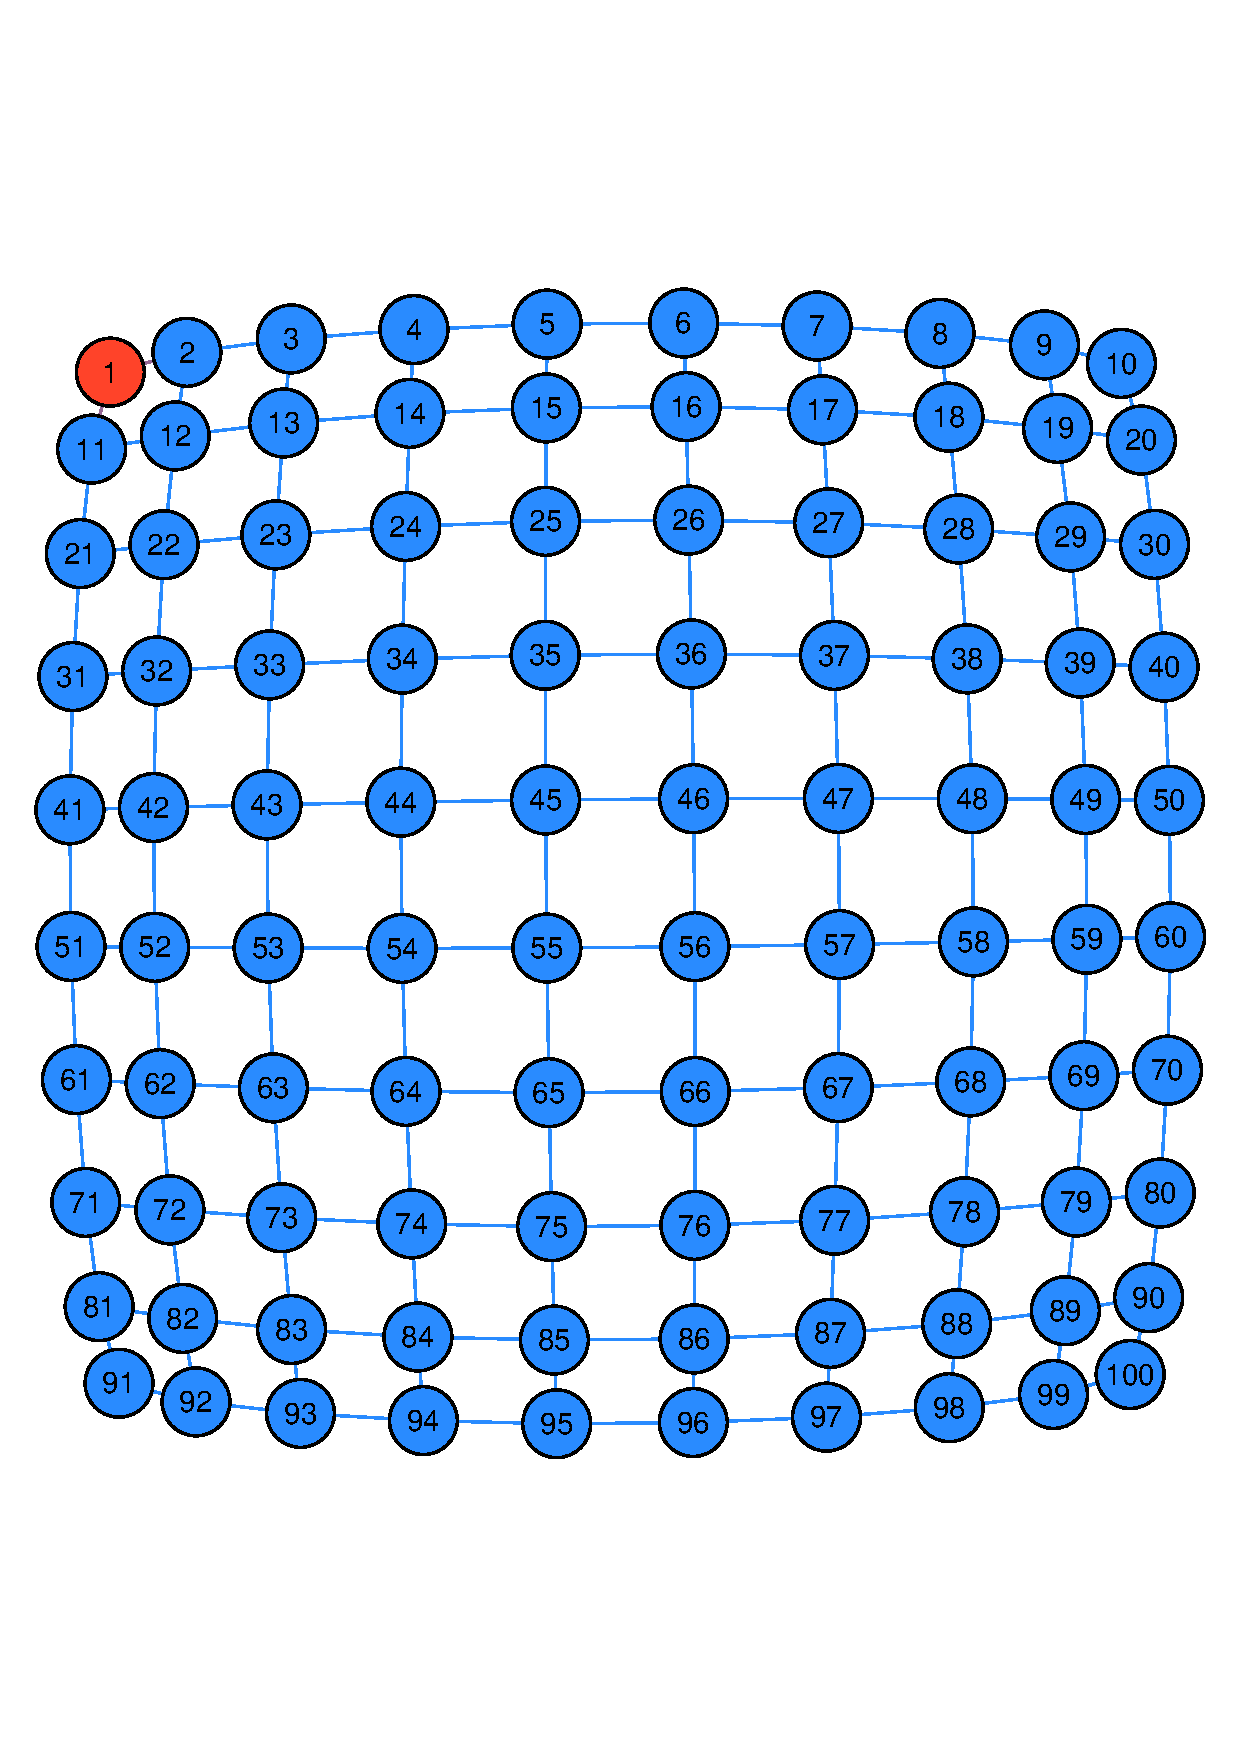
\includegraphics[width=\textwidth]{grid_start.pdf}
        \label{fig:start_grid}
	\end{subfigure}
 	\begin{subfigure}[b]{0.49\textwidth}
    	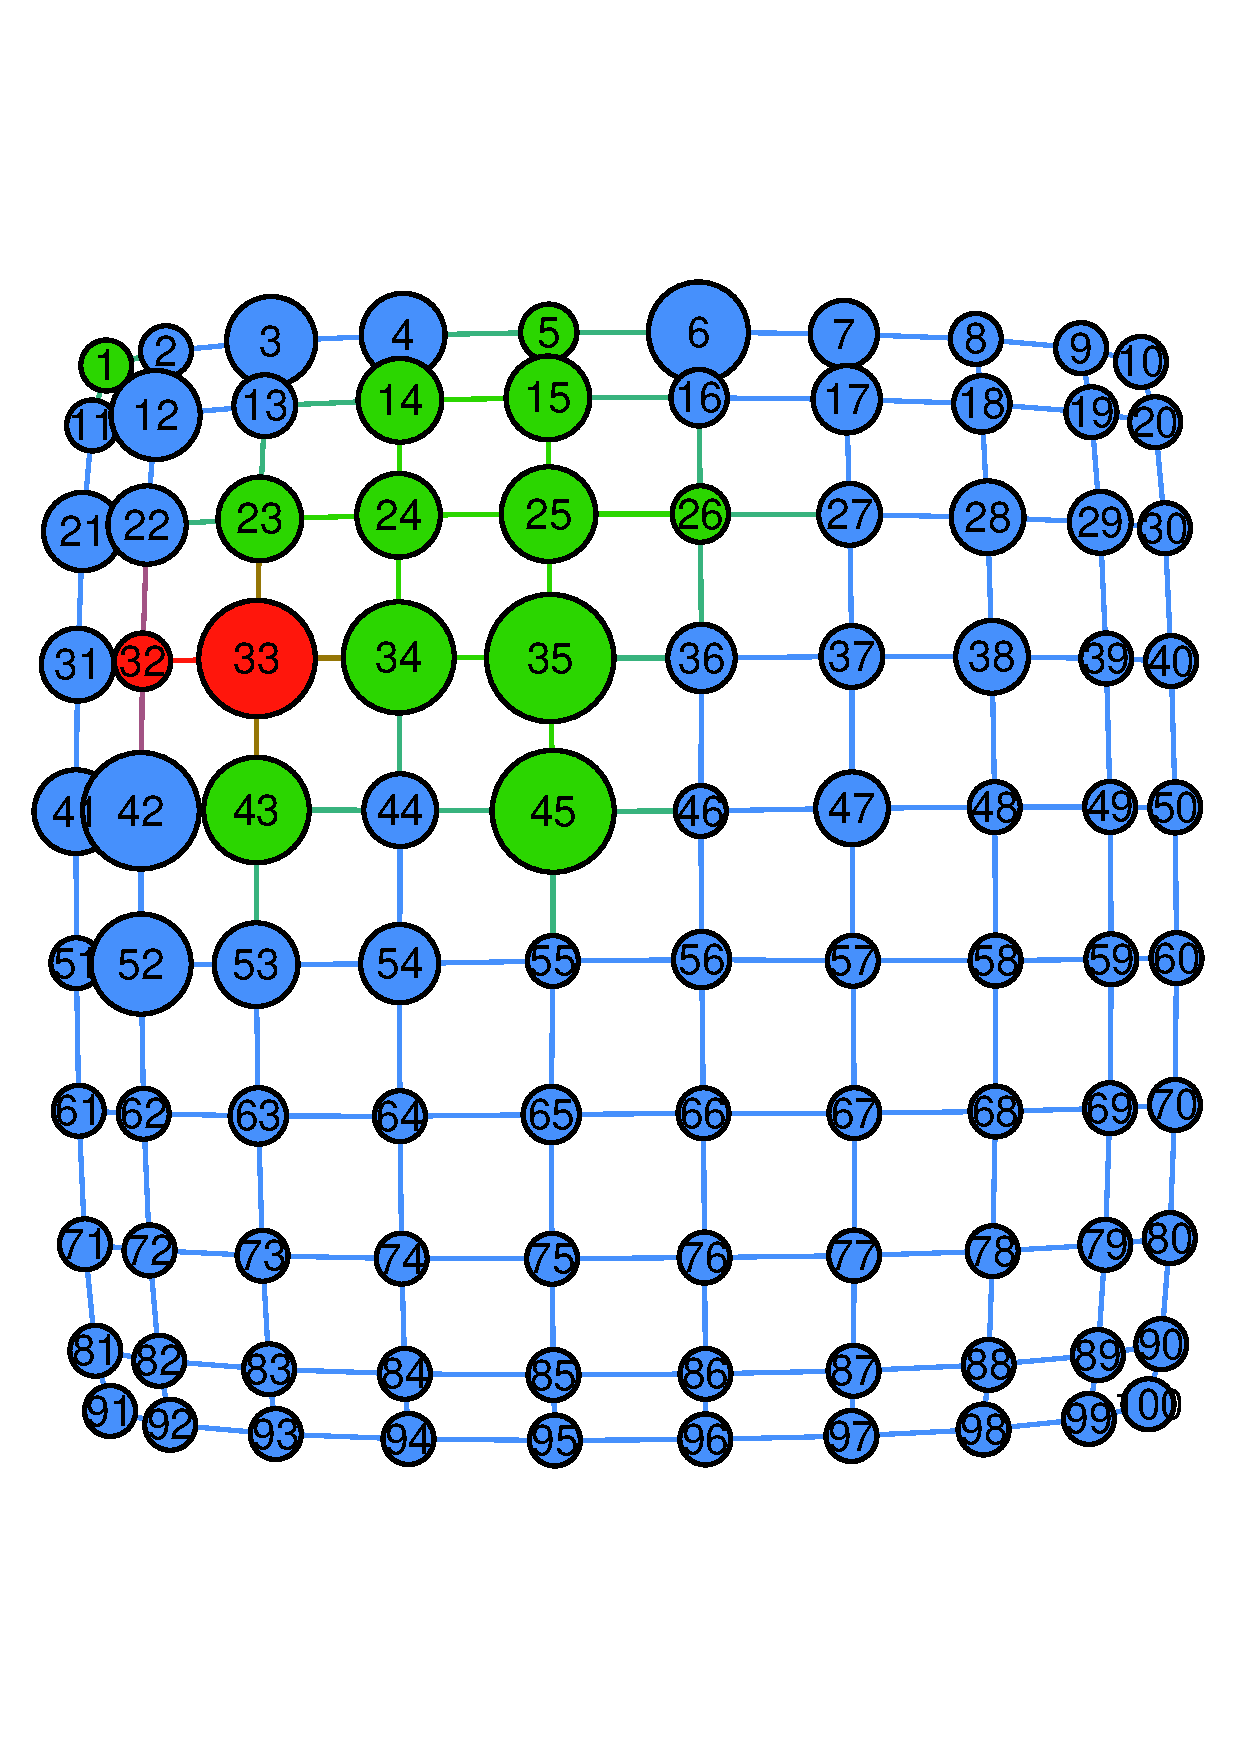
\includegraphics[width=\textwidth]{grid_run.pdf}
        \label{fig:running_grid}
	\end{subfigure}
    \caption{\textbf{Network structure used for simulations} The simulations were run on this grid like network comprised of 100 nodes. Infected nodes \textit{red}, susceptible nodes \textit{blue}, recovered nodes \textit{green} \textbf{Left:} This grid is in the very first time step which is the same for all simulations performed: Only one node is infected and all others are susceptible \textbf{Right:} The state of the network in the midst of an epidemic. The size of the nodes corresponds to its general awareness, e.g 0.875 for node 35 and 0 for node 100. Model parameters were $ \beta$=0.5 , $ \gamma$=0.4 , $ \alpha$= 0.6, $ \tau$=0.5 }
    \label{fig:grid}
\end{figure*}

\paragraph*{Input to the model / Model calibration} Equations \ref{eq:omega} - \ref{eq:tau} show and explain the $7$ defining parameters for our model. To study the impact of a certain parameter, the simulational outcome has to be compared for different values of this parameter, but also how it depends on the remaining parameters. On the other hand, parameter values can be chosen to fix the model behavior. For this work, it was the authors choice to fix large parts of the model to reduce complexity.\\
\begin{itemize}
 \item Perturbations: We assume a {\it uniform} distribution of random links throughout the population, i.e. each agent shares the same probability $\tau$ to be picked for establishing a random link in addition to its neighbors on the grid.
  \item Information generation: The probability $\omega$ of information being generated in case of an infection is fixed to $1.0$, i.e. for sure.
  \item Information radius: Information about each node is propagated over no more than $3$ edges to reduce run-time of our simulation.
  \item Decay of awareness: The decay rate $m$ of awareness is chosen to be $1/2$, i.e. $2$ unit-time after information was generated or propagated it has faded away.
  \item Authenticity of knowledge/awareness: For the damping of information over distance, cf. Equation \ref{eq:cutoff}, we chose $k = \log(2)$, i.e. the magnitude of knowledge is reduced by a factor of $1/2$ each time it is propagated.
\end{itemize}


\subsection{Metrics}
In each unit-time step, the current number of susceptibles as well as the number of recovered nodes is recorded for later analysis, from which we can easily derive the number of infected nodes in each unit-time step.
However, defining a single characteristic for the outcome of a simulation with certain parameters was found to be non-trivial.
The basic reproduction number $R_{0}$ commonly used as such---where $R_{0} > 1$ describes an epidemic---is not applicable to closed networks, as the mean number of secondary infections converges to $1$ when a large fraction of the population is infected and only few individuals stay susceptible.

\begin{itemize}
  \item Tuning: As metric for an epidemic outcome, we chose the mean number of cases, i.e. the integrated number of infections. The decision threshold for an uncontained epidemic is at $50 \%$ of the population in the last step.
\end{itemize}

\section{Simulation Results and Discussion}

%When related to, or combined with, real data, numerical simulations allow for {\it quantitative} analysis of the modelled states and their evolution at a level of detail that is beyond the richness of collectable data. At the same time, numerical simulations also allow for {\it qualitative} insights into several implications above the level of the underlying dynamics.
In the following, we present a qualitative analysis of some insights that we gained during the course of our simulations. In particular, we will focus on the disease dynamics with and without random links (perturbations), and we compare our model to a slightly modified one which uses divergent but static contact and information networks, i.e. the contact network is perturbed at the beginning and kept in this state during a complete run. Under some simplifying assumptions, we tuned our model to a certain number of cases of a disease in case of no perturbation. Fixing our model to these parameters, we then analyzed the impact of both varying the probability of random links and the probability of information spread on the number of cases of the modelled disease. As one would expect, by increasing perturbation, the modelled disease is generally more likely to show higher numbers of cases, while increasing the propagation of awareness reduces the numbers of cases, and both processes are therefore competing with each other. This section presents detailed analysis of data we obtained from our implementation of our model and discusses our results from these different perspectives. For more details on our simplifying assumptions we refer to the implementation part of this report.


\begin{figure*}[t]
	\centering
	\begin{subfigure}[t]{0.535\textwidth}
    	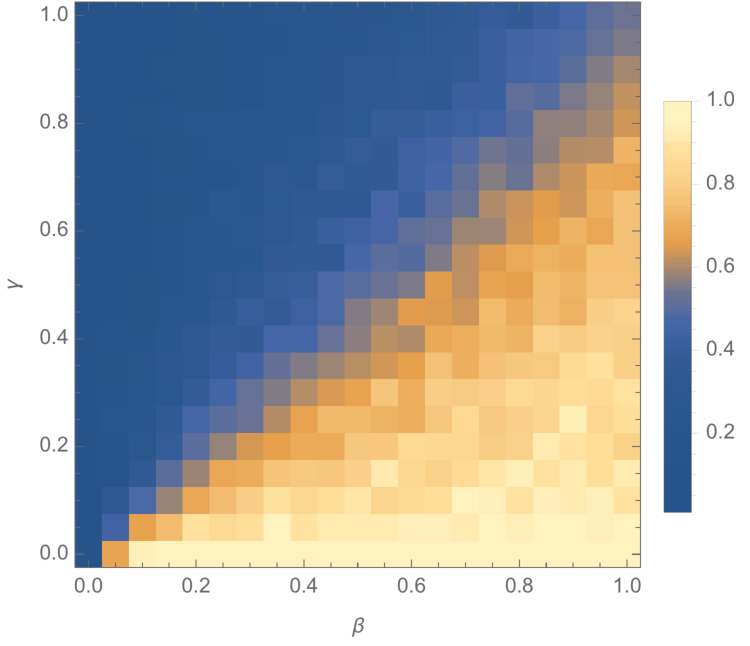
\includegraphics[trim = 0mm 2mm 0mm 0mm, clip, width=\textwidth]{beta_gamma_omega1_alpha0_tau0_expk2_runs50_nocut_notitle.pdf}
        \label{fig:beta_gamma_nocut}
        \caption{Density plot}
	\end{subfigure}
 	\begin{subfigure}[t]{0.45\textwidth}
    	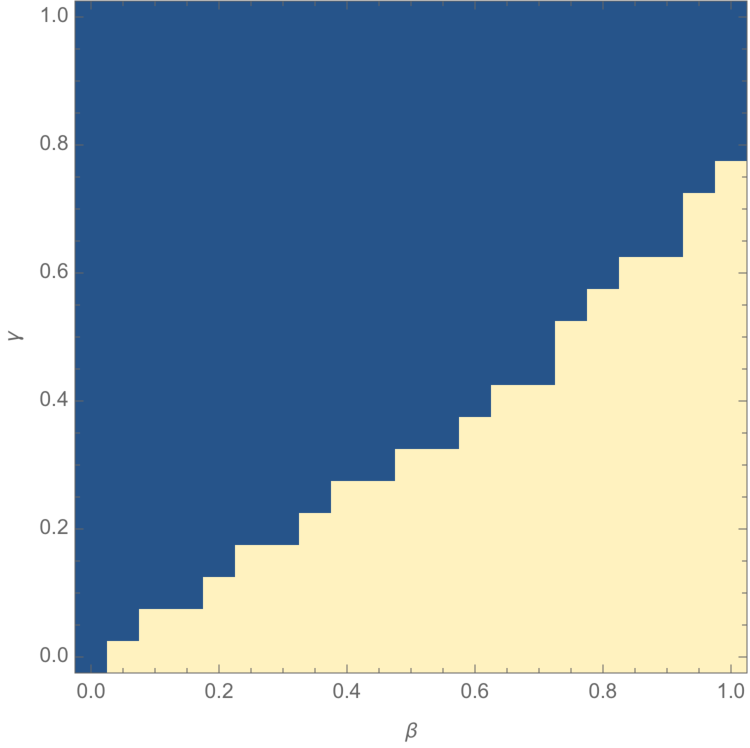
\includegraphics[width=\textwidth]{beta_gamma_omega1_alpha0_tau0_expk2_runs50_cut05_notitle.pdf}
        \label{fig:beta_gamma_cut}
        \caption{Density plot with threshold 0.5}
	\end{subfigure}
    \caption{\textbf{Epidemic outcome for $(\beta,\gamma)$ parameters.} Epidemic outcome, expressed as the fraction of total infections at the end of every simulation depending on $\beta,\gamma$ given $\alpha=0$, $\tau=0$, averaged over 50 simulations. \textit{Yellow:} More than 50\% of the population were infected. \textit{Blue:} More than 50\% remain susceptible.}
    \label{fig:beta_gamma}
\end{figure*}


\begin{figure*}[t]
	\centering
	\begin{subfigure}[b]{0.535\textwidth}
    	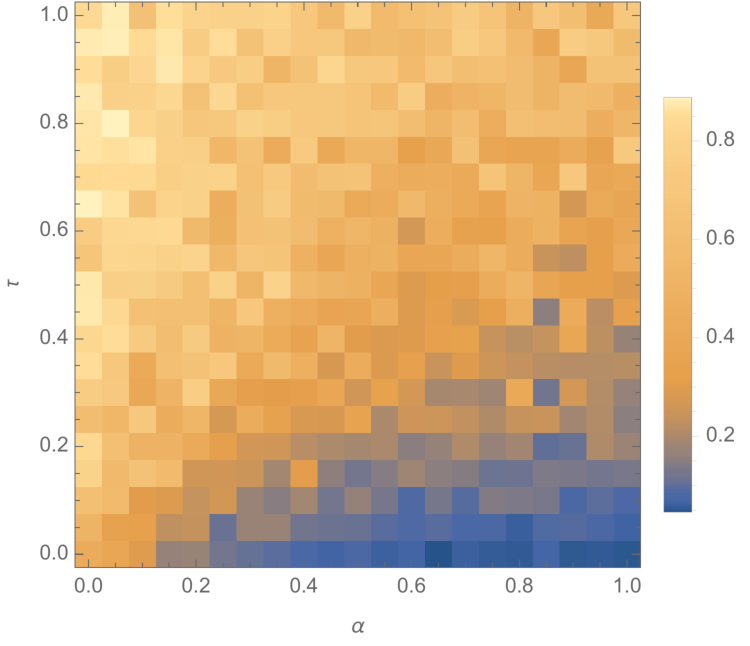
\includegraphics[trim = 0mm 2mm 0mm 0mm, clip, width=\textwidth]{alpha_tau_omega1_beta05_gamma03_expk2_runs50_nocut_notitle.pdf}
        \label{fig:alphataunocut}
        \caption{Density plot}
	\end{subfigure}
 	\begin{subfigure}[b]{0.45\textwidth}
    	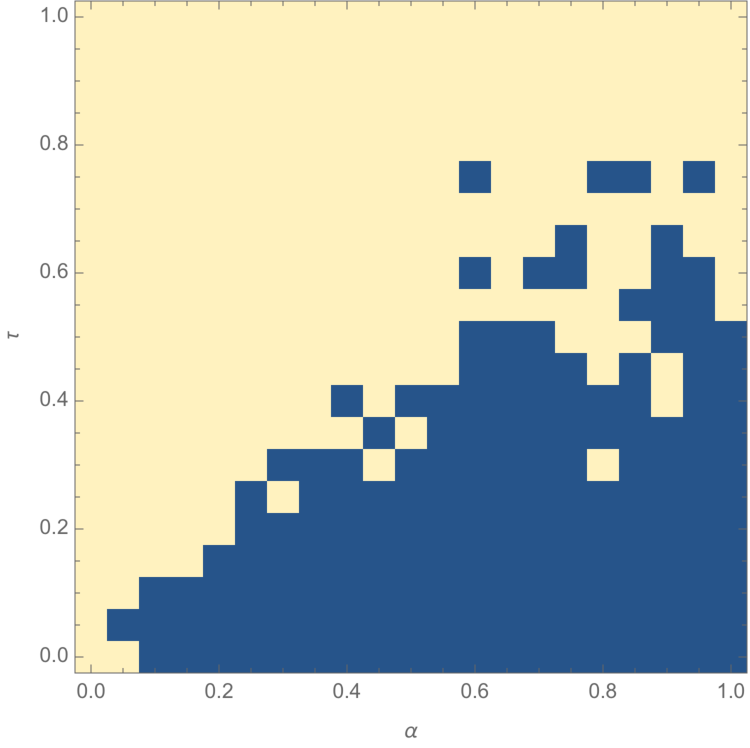
\includegraphics[width=\textwidth]{alpha_tau_omega1_beta05_gamma03_expk2_runs50_cut50_notitle.pdf}
        \label{fig:alphataucut}
	    \caption{Density plot with threshold 0.5}
	\end{subfigure}
    \caption{\textbf{Epidemic outcome for $(\alpha,\tau)$ parameters.} Epidemic outcome, expressed as the fraction of total infections at the end of every simulation depending on $\alpha,\tau$ given $\beta_{0}=0.5$, $\gamma_{0}=0.3$, averaged over 50 simulations.\textit{Yellow:} More than 50\% of the population were infected. \textit{Blue:} More than 50\% remain susceptible.}
    \label{fig:alphatau}
\end{figure*}


\begin{figure*}[t]
	\centering
	\begin{subfigure}[b]{0.78\textwidth}
    	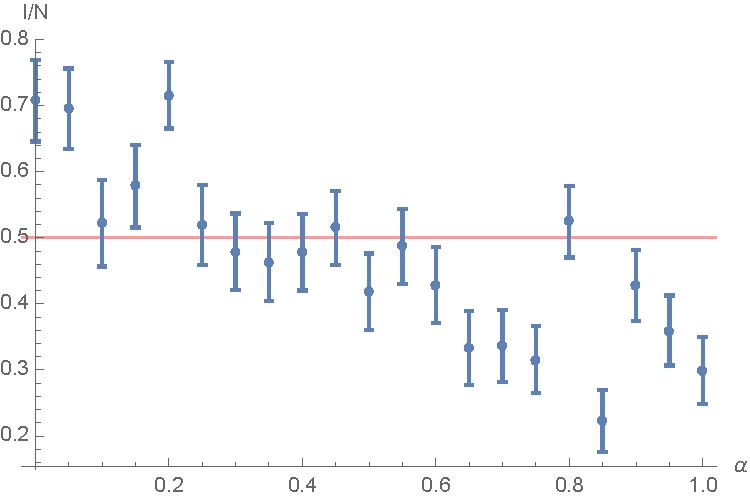
\includegraphics[width=\textwidth]{Itot_alpha_tau03_omega1_beta05_gamma03_expk2_runs50_notitle.pdf}
        \label{fig:itotalpha}
        \caption{$\tau$ = 0.3}
	\end{subfigure}
 	\begin{subfigure}[b]{0.78\textwidth}
    	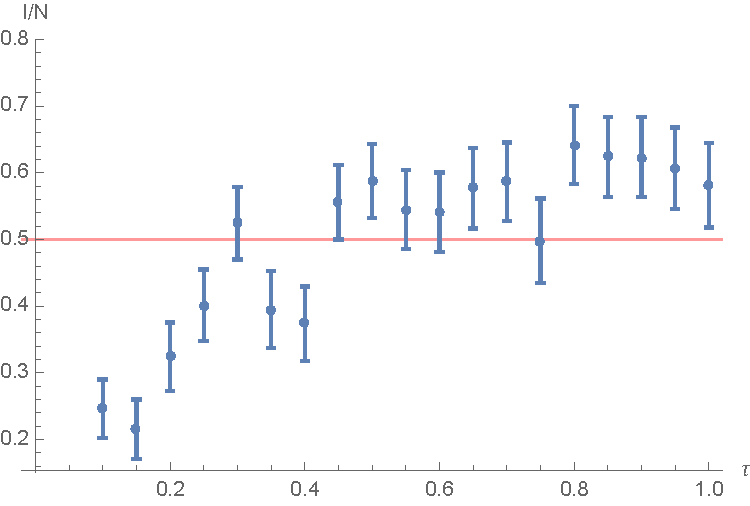
\includegraphics[width=\textwidth]{Itot_tau_alpha08_omega1_beta05_gamma03_expk2_runs50_notitle.pdf}
        \label{fig:itottau}
        \caption{$\alpha$ = 0.8}
	\end{subfigure}
    \caption{\textbf{Epidemic outcome for $\alpha$, respectively $\tau$ parameters.} Epidemic outcome, expressed as the fraction of total infections at the end of every simulation depending on $\alpha$, respectively $\tau)$ given $\beta_{0}=0.5$, $\gamma_{0}=0.3$, averaged over 50 simulations and 1-$\sigma$ intervals as error bars. These Figures represent cuts through the plots of Figure \ref{fig:alphatau}. \textit{Red line:} Threshold for epidemic outcome; 50\% of the population were infected.}
    \label{fig:itot}
\end{figure*}


\subsection{Balance between perturbation and information spread}

While not following the intuitive path, we start with a presentation of our findings on the dependency between the $\alpha$ and $\tau$ parameters, that is, the probabilities of information to be propagated along the information network and of a single node being picked for establishing a random link. For this purpose we fixed our parameters to $50 \%$ mean total infections during a simulation when turning off random links and information propagation. Using the acquired parameters $(\beta,\gamma)$ we swept through the complete $(\alpha,\tau)$ parameter space. While our results were quite expected, still, we observed some kind of unpredictable behavior for certain values of $(\alpha,\tau)$ which we attribute to instabilities of the resulting system.

\paragraph{Method}
Given aforesaid assumptions, we swept through all possible values of $0 \leq \beta \leq 1$ and $0 \leq \gamma \leq 1$ in steps of $0.05$, that is, the probabilities of contact (i.e. infection to spread along an edge in the contact network) and recovery per unit-time step. Also, we fixed the probabilities $\alpha$ and $\tau$ of information propagation and random linking per unit-time step to $0$, such that awareness is confined to the infected nodes themselves and there do not exist any random links.

From the resulting density plot we picked parameters $(\beta_0,\gamma_0)$ for which we then swept through all possible values of $0 \leq \alpha \leq 1$ and $0 \leq \tau \leq 1$.

\paragraph{Results}
%\todo{deviation in beta/gamma from first bsiecting -> awareness of infected node, in first step after self-infection only half prob to infect someone else}

Figure \ref{fig:beta_gamma} shows the distribution of mean total infections for each set of $(\beta,\gamma)$. The regions below and above threshold, as defined before, are separated roughly along the first bisecting line but trending for lower values at higher $\beta$. For $\gamma \geq 0.8$ more than half of the population is infected regardless of the value of $\beta$.

We have then chosen $(\beta_0,\gamma_0) = (0.5,0.3)$ for which the mean total number of infections is just below the threshold. The resulting density plot is shown in Figure \ref{fig:alphatau}. The region above threshold is found towards high values of $\tau$ and low values of $\alpha$, while for high values of $\alpha$ and low values of $\tau$ the mean of total infections is generally below threshold. In contrast to the $\beta/\gamma$ density plot, in the $\alpha/\tau$ density plot both phases are only irregularly separated and for higher values of $\alpha$ we find instability between both phases. To investigate this issue, we plotted the mean number of total infections for a fixed number of $\alpha$ and $\tau$ respectively, i.e. those plots represent a cut through the density plot. The resulting plots are seen in Figure \ref{fig:itot} for $\tau = 0.3$ and for $\alpha = 0.8$. We can see that both plots show statistically significant non-stable behavior, in the sense of Lipschitz-continuity. Remarkable points in the selected plots are $\tau = 0.3$, $\tau = 0.75$, $\alpha = 0.2$, and $\alpha = 0.8$.

\paragraph{Discussion}
We conclude that, as expected, with higher numbers of random links, more people are likely to be infected. This effect can be generally compensated with higher probabilities of information propagation, that is, increasing the speed of the information front. For high $(\alpha,\tau)$ values we generally find instability in the sense that the system becomes unpredictable (noncontinuous).

More data is needed to investigate these hot-spots.


\begin{figure*}[t]
	\centering
	\begin{subfigure}[b]{0.49\textwidth}
    	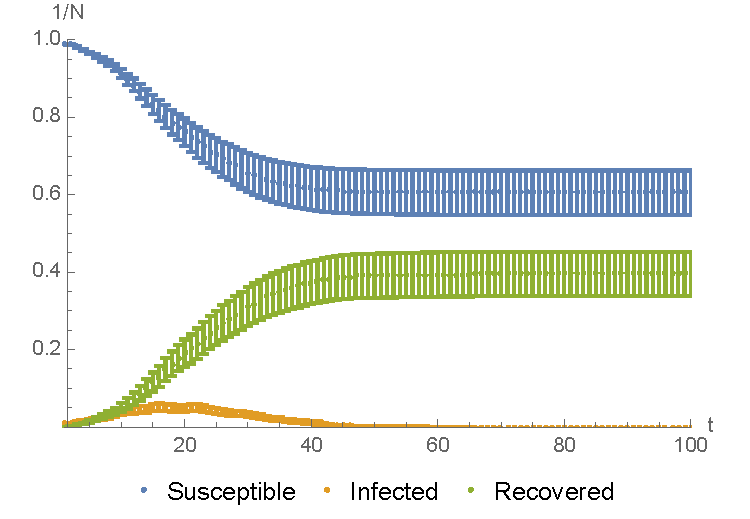
\includegraphics[width=\textwidth]{sir_alpha08_tau035_omega1_beta05_gamma03_expk2_runs50_notitle.pdf}
        \label{fig:sir_8035}
        \caption{$\alpha=0.8, \tau=0.35$}
	\end{subfigure}
	\begin{subfigure}[b]{0.49\textwidth}
    	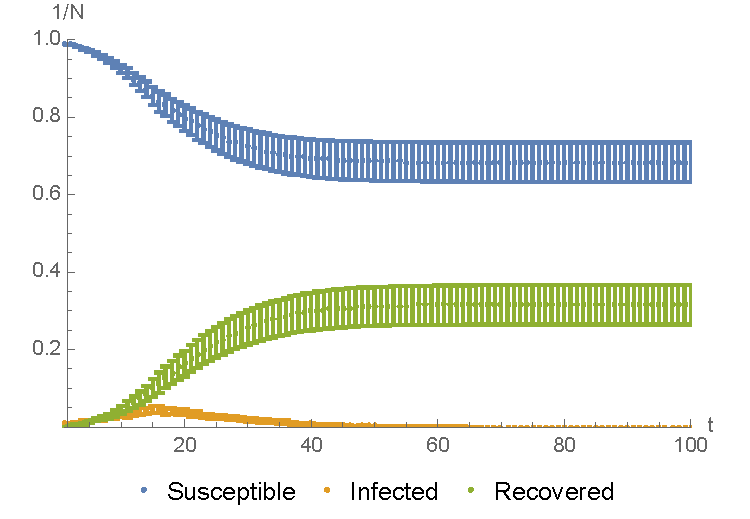
\includegraphics[width=\textwidth]{sir_alpha075_tau03_omega1_beta05_gamma03_expk2_runs50_notitle.pdf}
        \label{fig:sir_7530}
        \caption{$\alpha=0.75, \tau=0.3$}
	\end{subfigure}
	\begin{subfigure}[b]{0.49\textwidth}
    	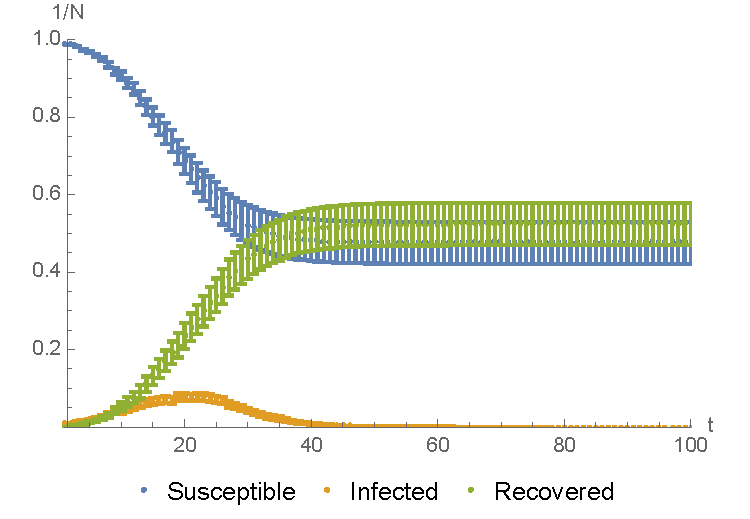
\includegraphics[width=\textwidth]{sir_alpha08_tau03_omega1_beta05_gamma03_expk2_runs50_notitle.pdf}
        \label{fig:sir_8030}
        \caption{$\alpha=0.8, \tau=0.3$}
	\end{subfigure}
	\begin{subfigure}[b]{0.49\textwidth}
    	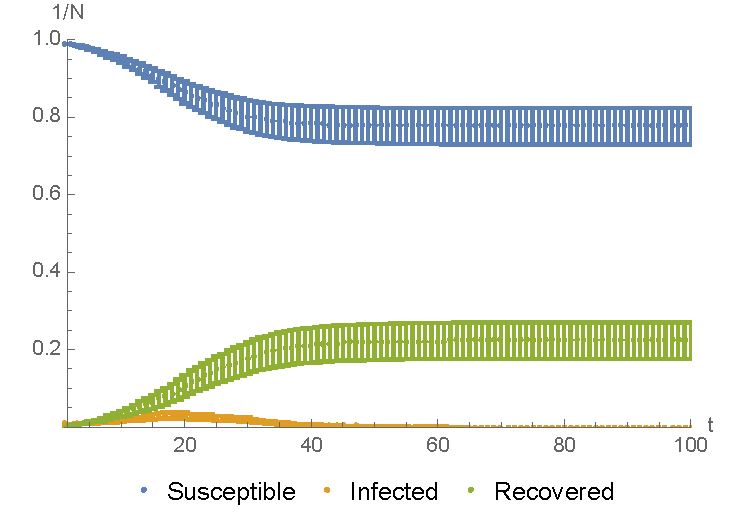
\includegraphics[width=\textwidth]{sir_alpha085_tau03_omega1_beta05_gamma03_expk2_runs50_notitle.pdf}
        \label{fig:sir_8530}
        \caption{$\alpha=0.85, \tau=0.3$}
	\end{subfigure}
	\begin{subfigure}[b]{0.49\textwidth}
    	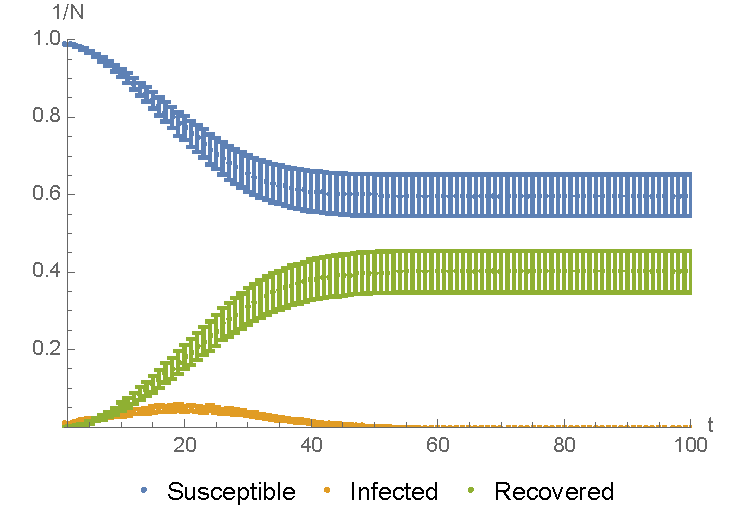
\includegraphics[width=\textwidth]{sir_alpha08_tau025_omega1_beta05_gamma03_expk2_runs50_notitle.pdf}
        \label{fig:sir_8025}
        \caption{$\alpha=0.8, \tau=0.25$}
	\end{subfigure}
    \caption{\textbf{SIR plots} The fraction of the population in each of the SIR compartments during the simulations for different values of $\alpha$ and $\tau$ given $\beta_{0}=0.5$, $\gamma_{0}=0.3$, averaged over 50 simulations and 1-$\sigma$ intervals as error bars.}
    \label{fig:sir}
\end{figure*}


\subsection{Prevalence and dynamics of the disease}

We found that introduction of random links not only changes the mean number of total infections but also influences the prevalent time of the disease. To make this effect more tangible, we created several SIR plots to illustrate this effect, and we provide an intuitive explanation based on the picture of propagating fronts.

\paragraph{Method}
From the data collected before, we can also generate conventional SIR plots which depict, for each unit-time step, the mean fraction of the population that is in either one of the compartments.

\paragraph{Results}
The resulting plots around the interesting hot-spot $(\alpha,\tau) = (0.8,0.3)$ with $(\beta_0,\gamma_0) = (0.5,0.3)$ are shown in Figure \ref{fig:sir}. In accordance with our findings before, we can see that for $(\alpha,\tau)$ values slightly lower/greater than the hot-spot values, the peak of the infected fraction in the population is generally more flat and, in the case of $\alpha = 0.75$, also significantly shorter. The latter finding is, in particular, also in accordance with other data not included in this report.

\paragraph{Discussion}
We conclude that the variation in information spread does not only influence the mean number of total infections in the sense that it flattens the distribution of the infected fraction in the population, but information spread also affects the prevalent time during which the disease is present in the population. We suggest the following---hand-wavy---explanation: Without random links, for appropriate values of $\beta$ and $\alpha$, the information front is running ahead of the infection front and, considering the decay of awareness over time and distance, the information becomes ineffective. Now, by perturbing the contact network, on one hand, the disease can reach nodes outside of the infected nodes' neighborhoods and in particular before information reaches, but in contrast to the case before, two wave-fronts of infection and information are running through the population, colliding at some point and thus effectively impeding the spreading of the disease.

It would be interesting to analyze the reproduction rate of a disease for different values of $\alpha$. However, we found that due to our network being closed (no births, no deaths), the reproduction number will almost always converge towards $1$ by the end of a simulation and is therefore an inappropriate measure for our assumptions.

Again, more data is needed to investigate this issue.


\begin{figure*}[t]
	\centering
	\begin{subfigure}[b]{0.535\textwidth}
    	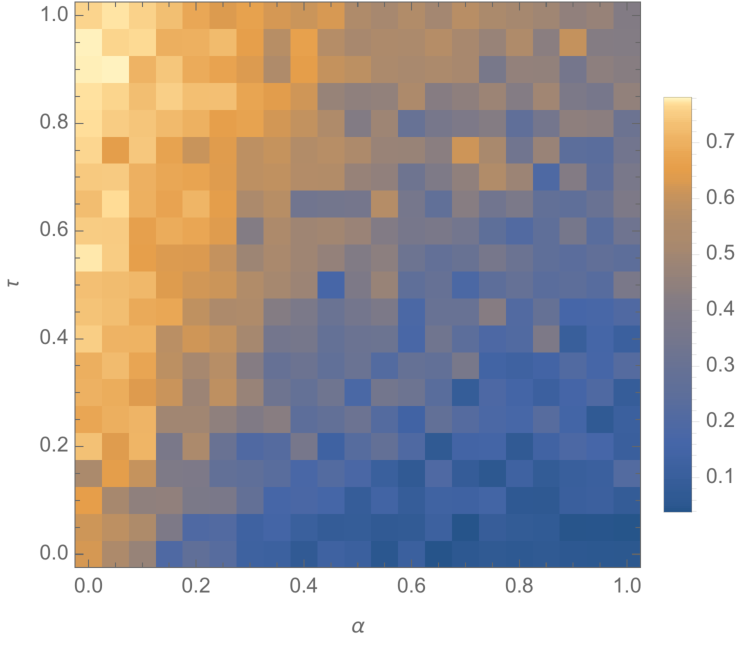
\includegraphics[trim = 0mm 2mm 0mm 0mm, clip, width=\textwidth]{alpha_tau_static_omega1_beta05_gamma03_expk2_runs50_nocut_notitle.pdf}
        \label{fig:alphatau_static_nocut}
	\end{subfigure}
 	\begin{subfigure}[b]{0.45\textwidth}
    	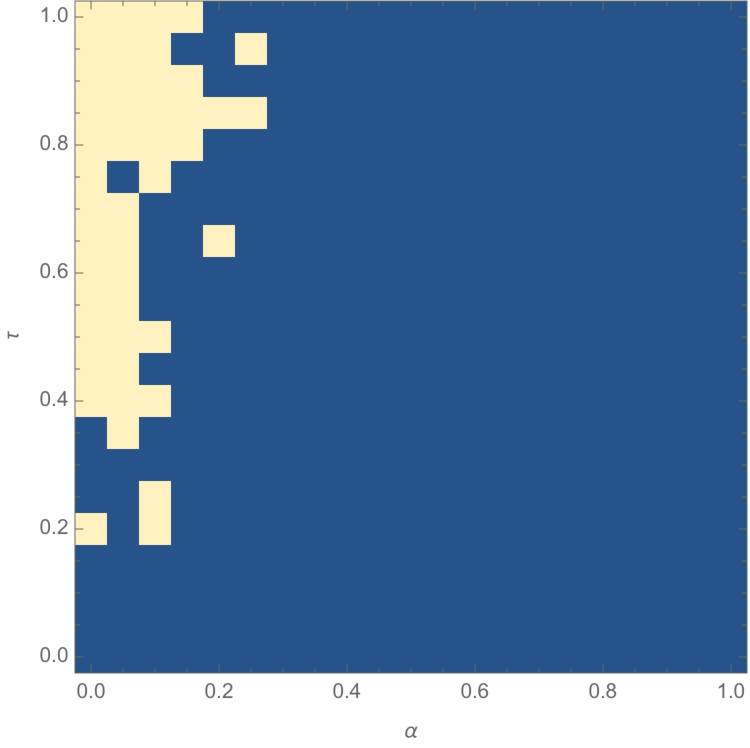
\includegraphics[width=\textwidth]{alpha_tau_static_omega1_beta05_gamma03_expk2_runs50_cut05_notitle.pdf}
        \label{fig:alphatau_static_cut}
	\end{subfigure}
    \caption{\textbf{Epidemic outcome for the case of static divergent contact and information networks for $(\alpha,\tau)$ parameters.} Random links in the contact network governed by $\tau$ are only once generated and are stable. Epidemic outcome, expressed as the fraction of total infections at the end of every simulation depending on $\alpha,\tau$ given $\beta_{0}=0.5$, $\gamma_{0}=0.3$, averaged over 50 simulations.\textit{Yellow:} More than 50\% of the population were infected. \textit{Blue:} More than 50\% remain susceptible.}
    \label{fig:alphatau_static}
\end{figure*}


\subsection{Comparison with static divergent networks}

We were also interested in whether our simulation shows different dynamics than a similar model with divergent contact and information frameworks, and without perturbation ("static divergent"). Modifying our implementation towards static divergent networks, we compare the resulting $(\alpha,\tau)$ density plot to the one obtained before. We find that both models exhibit different behavior.

\paragraph{Method}
Our implementation was slightly modified to perturb the contact network only at the beginning of each run but not {\it during} each run. Using this modified model, we again carried out our analysis of the $(\alpha,\tau)$ parameter space.

\paragraph{Results}
Figure \ref{fig:alphatau_static} shows the resulting $(\alpha,\tau)$ density plot for our {\it static divergent} model analogous to Figure \ref{fig:alphatau} before. We can observe the same fundamental behavior: Increasing number of infections for high values of $\tau$ and decreasing number of infections for high values of $\beta$. In contrast to our original model, the spread of awareness seems to dominate the process in the sense that only for high $\tau \geq 0.4$ and exceptionally low $\alpha \leq 0.2$ the mean number of infections crosses our threshold.

\paragraph{Discussion}
We conclude that our model is a generalization to the conventional stochastic SIR model coupled to an information network with possibly divergent but static contact and information networks. However, we are missing metrics to quantity and assess this "level of generalization".

More analysis needs to be carried out to investigate these differences.


\subsection{Limitations}

Having stated our findings before, we need restrict our results with the following remarks. They primarily concern our simplifying assumptions:

\begin{itemize}
  \item Topology: Our choice of topology is completely arbitrary and artificial. In particular, grid-type networks do not exhibit features of real social networks as would be appropriate when treating {\it social} discovery. Also, the small number of simulated nodes does not allow for practicable conclusions towards real-world diseases. Instead, our network choice was led by ease-of-implementation and low run-time requirements. Additionally, depending on a specific disease to be modelled, one should also consider open networks.
  \item Perturbations: A uniform distribution of random contact probability does not reflect real-world conditions at all. Instead, it should be assumed, that just a small fraction of the population is engaging in random contacts frequently, while the vast majority does not make use of social discovery at all (until today).
  \item Awareness: Our choices for the time-decay rate $m$ of knowledge/awareness and its distance-dependency characterized by $k$, are, again, completely arbitrary. In particular, interpretation of the decay rate makes only sense together with the all the other probabilities defined on a time step. After all, the practical significance of a {\it unit}-time step has not been treated in this work.
  \item Information radius: Similarly as for the awareness part, our choice of the information radius is completely arbitrary. Furthermore, we did not investigate to what extent different values for the radius do influence the outcome of our simulations. This issue, again, asks for more detailed treatment.
  \item Disease Traits: Our model accounts only for diseases where the contact network basically equals the information network. However, for diseases like STDs where the contact network is only a small subset of the information network, perturbations are not able to mimic the dynamics.
\end{itemize}


\section{Summary and Outlook}


\subsection*{Summary}

We defined a model for the spread of infectious diseases when considering random links from social discovery. For this purpose, we imagine social discovery as short-term perturbations to the otherwise static contact network along which the disease spreads, while assuming that information spreads strictly along the static part of the contact network. Our proposed model extends the conventional stochastic (agent-based) SIR model with spread of awareness (as done before in \citep{Funk}) and with short-term perturbations of the contact network. In particular, our model differs in 2 aspects from existing works: First, the contact network changes within each unit-time step. Secondly, for this reason, information is generated at different locations in the network in the sense that multiple information fronts emerge. Our own implementation of this model was done completely from scratch and in Matlab. We then analyzed three different aspects of our simulation: (1) How does our model compare to similar, existing model with divergent, yet static contact and information networks? We found that, while exhibiting similar fundamental features, our model comes up with different data. We attribute this observation to the short life span of the divergent links in both networks. (2) Does, and if so, how does the introduction of random links change the dynamics of an epidemic outbreak? Regarding this question, we found out that introduction of (additional) random links does not only increase the number of infections---as one would probably expect---but also the prevalent time of the disease in the population may be reduced under certain circumstances. (3) How are information spread and random links related? We found out that, generally and as expected, with higher probabilities for random links, the number of infections is {\it in}creasing, while with higher probability of information propagation the number of infections is {\it de}creasing, and consequently, both processes are competing with each other. For high probabilities of random links as well as of information propagation we found that the outcome of the system becomes more and more unpredictable (in the sense of less Lipschitz-continuous). However, all these findings are based on several fairly ambiguous and artificial assumptions and all of these effects ask for more detailed investigation which was out of scope for this project.


\subsection*{Outlook}

As stated in the section before, several options can be considered for future work on our type of model. Most options concern our choice of assumptions. Generally, our simulation should be tested for larger parameter spaces which at the same time will increase run-time of the simulations significantly. In addition to the remarks made before, following extensions seem particularly interesting:

\begin{itemize}
  \item Statistics: For the sake of completeness, one should repeat our simulations using a different random number generator to check against hidden correlations.
  \item Information generation: In this work, we did not consider the information generation probability $\omega$ at all. Instead, we just assumed that information is always generated. However, this parameter allows for simulation of a different class of diseases: As an alternative to the epidemiological SEIR model, asymptomatic individuals can be readily treated in our model by tuning the $\omega$ parameter. Also, one could consider a time-dependent $\omega(t)$ parameter.
  \item Perturbations: While our implementation already allows for distributions of $\tau_i$ per node, it does not treat spatial distance yet. Take for example Tinder, where there exists a spatial distance criterion to find new contacts. In the same sense, our model does not distinguish between random contacts in one node's close neighborhood---it is equally possible to establish a random contact with an immediate neighbor. More careful treating of the perturbation part of our model seems therefore appropriate. Another possible extension concerns the life-span of a random link assumed to be identical to a unit-time step so far which could be randomized similar to the recovery probability.
\end{itemize}


\bibliographystyle{plainnat}
\bibliography{Transmissionary}


\end{document}
